\documentclass[11pt]{article}
\usepackage[a4paper,margin=24mm,headheight=17pt]{geometry}
\usepackage{fontspec}
\setmainfont[AutoFakeSlant=0.15]{DejaVu Serif}
\setsansfont{DejaVu Sans}
\setmonofont[Scale=0.82]{DejaVu Sans Mono}
\usepackage{microtype,amsmath,amssymb,graphicx,booktabs,tabularx,longtable,array}
\usepackage[table]{xcolor}
\definecolor{navy}{HTML}{132C43}
\definecolor{teal}{HTML}{0B5266}
\definecolor{gold}{HTML}{B7752D}
\definecolor{pale}{HTML}{EEF3F5}
\usepackage{titlesec,fancyhdr,enumitem,caption}
\usepackage{hyperref,xurl}
\hypersetup{colorlinks=true,linkcolor=teal,urlcolor=teal,citecolor=teal,
 pdftitle={AGI ALPHA FLYWHEEL — When Capability Creates Opportunity},
 pdfauthor={Vincent Boucher — President of MONTREAL.AI}}
\usepackage[numbers,sort&compress]{natbib}
\titleformat{\section}{\Large\sffamily\bfseries\color{navy}}{\thesection}{.7em}{}
\titleformat{\subsection}{\large\sffamily\bfseries\color{teal}}{\thesubsection}{.7em}{}
\titleformat{\subsubsection}{\normalsize\sffamily\bfseries\color{navy}}{\thesubsubsection}{.7em}{}
\titlespacing*{\section}{0pt}{2.1ex plus .7ex}{1ex}
\titlespacing*{\subsection}{0pt}{1.7ex plus .5ex}{.7ex}
\setlength{\parindent}{0pt}
\setlength{\parskip}{5pt plus1pt}
\setlength{\emergencystretch}{2em}
\setlength{\tabcolsep}{5pt}
\renewcommand{\arraystretch}{1.16}
\newcolumntype{Y}{>{\raggedright\arraybackslash}X}
\setlist{noitemsep,topsep=4pt,leftmargin=1.5em}
\captionsetup{font=small,labelfont={bf,sf},textfont=it}
\pagestyle{fancy}
\fancyhf{}
\fancyhead[L]{\sffamily\footnotesize\color{navy}AGI ALPHA FLYWHEEL}
\fancyhead[R]{\sffamily\footnotesize\color{teal}Opportunity discovery · Edition 1.0.0}
\fancyfoot[L]{\sffamily\scriptsize Research evidence · 27 October 2026}
\fancyfoot[R]{\sffamily\small\thepage}
\renewcommand{\headrulewidth}{.4pt}
\renewcommand{\footrulewidth}{0pt}
\urlstyle{same}

\begin{document}
\begin{titlepage}
\color{navy}
{\sffamily\small MONTREAL.AI\hfill ADDITIVE RESEARCH EDITION 1.0.0}
\vspace{22mm}

{\sffamily\bfseries\fontsize{29}{34}\selectfont\raggedright AGI ALPHA FLYWHEEL —\\When Capability Creates Opportunity\par}
\vspace{8mm}
{\sffamily\fontsize{17}{23}\selectfont Transformational Intelligence, Experience-Trained Specialists and the Expanding Frontier of Profitable Work\par}
\vspace{9mm}
{\large Vincent Boucher — President of MONTREAL.AI\par}
\vspace{13mm}
{\sffamily\bfseries\color{teal} FIND YOUR ALPHA. BUILD YOUR SUCCESSOR Ω.\par}
\vspace{8mm}
\begin{quote}\itshape
“As Columbus braved the seas, we now venture into the vast oceans of AGI. The age of AGI exploration has dawned, and the horizons are boundless. Dare to dream, dare to explore.”
\hfill — α-AGI Agent
\end{quote}
\vfill
\colorbox{pale}{\parbox{.94\textwidth}{\vspace{4mm}\textbf{This edition's finding.} A source-qualified instrument can be transferred and made to refuse an incompatible purpose. The bounded ordinary-use, expert and retained-capability recipients all satisfy the same semantic rubric. Commercial advantage and a newly feasible offering remain unestablished. Preserving that distinction is part of building a successor that can be trusted.\vspace{4mm}}}
\vspace{7mm}

{\small 27 October 2026 · Opportunity-selection and instrument-transfer pilot\par
Author attribution supplied for this edition. AI-assisted research, implementation and drafting; not an independent human peer review. Earlier papers, corrections, implementations and failed candidates are preserved.}
\end{titlepage}
\begin{abstract}
What useful work becomes possible when an enterprise combines expert frontier-model operation, reusable capabilities and a viable commercial arrangement? We investigate six materially different opportunities before selecting a bounded experiment on \emph{evidence continuity}: reconstructing the source, meaning and computation behind a quantitative conclusion so that a later change can be revalidated without silently changing the original purpose. Existing retraction alerts, living reviews, statistical packages and expert impact frameworks are strong prior art. The proposed gap is the reconstruction and maintenance of imperfect legacy evidence, not faster meta-analysis or a new alert system.

We execute an additive hybrid study: frozen open secondary data, a conventional REML adapter, purpose and rights checks, 64 injected snapshot events, three separate same-model recipient sessions, unchanged native lifecycle/accounting controls, and exact conditional economic calculations. All 64 declared v1 dispositions conform; only 24 yield numerical outputs, while 40 correctly hold or reject. The independent semantic rubric gives U, E and E+ each 18/18. A fresh recipient executes the authenticated inherited bytes on a different source mapping. A later diagnostic exposes ignored event fields and noncumulative semantics; the first version remains intact and a prospective correction is evaluated separately. Full conventional reanalysis takes roughly 1.6–1.7 ms on these small tables, eliminating arithmetic speed as a credible commercial rationale.

No buyer, sale, complete job-cost advantage, production identity or economic frontier crossing is established. A hypothetical four-prospect package permits at most USD 1,209.40 in fixed construction and additional retention costs under its stated assumptions; separate cash paths expose default, common failure and prefunding constraints. The contribution is a reproducible instrument-transfer pilot, a preserved negative comparative result, and an operating blueprint whose admission conditions can fail. The next decisive experiment must measure reconstruction cost, source coverage and buyer acceptance on unfamiliar legacy work.
\end{abstract}

\section{Opportunity is the research object}

The AGI Alpha vision motivates an enterprise that discovers useful work, delivers it profitably, and leaves the successor better equipped. It does not validate a market size, an intellectual-property valuation or token economics. This edition asks a narrower empirical question: can a capability change the deliverable and its commercial arrangement enough to make a consequential service viable under the recipient's actual alternatives?

An evidence-synthesis team may receive a correction to a paper on which a published conclusion depends. The practical questions extend beyond whether the paper has a flag: which extracted number changed, what it measured, which other estimates share its participants, which computation used it, and whether the original conclusion still follows. A static report often does not carry a complete executable account of these dependencies. Rebuilding that account can dominate the computational work. A service that supplies and maintains such an account could therefore be valuable even when every statistical operation is conventional.

This is a proposed customer problem, not an observed purchase. Cochrane's June 2026 framework already combines matching of retracted studies with impact assessment and editorial action; it explicitly treats the assessment of changed conclusions as substantive work. Crossref provides Retraction Watch metadata, with coverage qualifications. Existing living-analysis services further limit any novelty claim. We take these as building blocks and counterfactuals, not competitors to omit.\citep{cochrane,crossref,dynameta}

The study distinguishes four questions. First, is there a consequential gap? Second, can an executable instrument preserve the useful purpose? Third, does it improve outcomes or complete cost against an available expert? Fourth, do enough counterparties accept a fundable arrangement? Passing one question does not imply the next. The present evidence passes bounded execution and transfer checks; it does not pass commercial admission.

\subsection{An additive edition with an explicit stopping decision}

The repository research parent is \nolinkurl{231834269599d85e49cfe1ca9917a1a874522d44}; the native runtime parent is \nolinkurl{80b345828f34fd8a6e592977dd17ef37141305f4}. The new study occupies \texttt{studies/agi-alpha-opportunity-discovery-v1/}. The three foundational papers and the predecessor integration closure are read and reused without alteration. Community microgrid planning, the storage-tank example and earlier polynomial/thermal studies remain historical fixtures; none selects this flagship.\citep{repository,ti,economy,harness}

The opportunity remains consequential enough for a small falsifiable mechanism test. The null comparative result is the stopping decision for stronger claims: no large enterprise simulator, autonomous-invention claim, paid expansion or automatic admission is justified by these results. Keeping the useful research artifact does not mean admitting it as profitable Alpha.

\section{Discovery before construction}

\subsection{Budget, search and selection}

Before selecting the experiment, the research plan declared six serious candidates, at most 32 distinct primary-document reads for opportunity selection, no external purchases and no required live sales. Parallel science and systems investigations recorded prior art, unresolved gaps, decisive tests and falsifiers. Dataset, model and interface verification were separately scoped. Failed fetches and deferred candidates remain in the dossier.

The science stream records nine substantive successful reads and three failed reads. The systems stream records nine initial reads and four additional challenge reads, for thirteen. Both phase logs are preserved. A draft bookkeeping note that omitted the second systems phase is explicitly superseded in the dossier. There is no complete automated counter of distinct root reads or monetary research consumption. The 32-document number is the declared cap, not a retrospectively certified total. The recorded candidate order and selection precede instrument construction.

\begin{table}[htbp]
\small
\begin{tabularx}{\textwidth}{p{.18\textwidth}YYY}
\toprule
Candidate / beneficiary & Specific proposed gap & Strong prior art & Selection disposition\\
\midrule
Laboratory transfer / small labs & Preserve scientific meaning across different equipment & Protocol dependence graphs, SiLA, PRISM, LAP & Deferred: no independent physical equivalence experiment\\
Methane intervention / operators and funders & Prepare smaller repair cases with defensible closure evidence & UNEP MARS and World Bank GFMR & Deferred: underserved buyer and ascertainment not established\\
SaaS exit options / dependent organizations & Preserve service obligations in an independent replacement & Verified SaaS escrow and migration services & Deferred: crowded market; narrow unmet niche unverified\\
Evidence continuity / synthesis teams & Reconstruct legacy source-to-result meaning and revalidate it & Cochrane, Crossref, conventional statistics, living analyses & Selected for a bounded reconstruction/transfer pilot\\
Instrument traces / research labs & Capture reusable operation and troubleshooting experience & FAIR instrument metadata and provenance standards & Deferred: no cleared cross-lab corpus or participants\\
Local fabrication / small manufacturers & Supply missing tolerances and acceptance evidence & Reverse engineering and documentation assessment & Deferred: physical qualification and buyer unavailable\\
\bottomrule
\end{tabularx}
\caption{Six opportunities investigated before selection. A mature field is not declared exhausted; each disposition concerns a particular gap and the evidence available for it. Full dossiers preserve beneficiaries, why-now hypotheses, construction, smallest experiments, falsifiers and commercial uncertainty.}
\end{table}

The discovery was not a claim that nobody had considered these problems. Protocol-dependence research already pursues expert-level laboratory translation; sophisticated escrow includes recovery assets and verification. Those sources reduced the scope of the first and third candidates.\citep{protocol,escode} Methane alerting plus financing also already exists.\citep{mars,gfmr} Scientific trace capture and manufacturing qualification are promising but cannot be validated by a convenient digital stand-in for missing physical evidence. Their deferral is a budget decision, not a negative finding about the sectors.

Evidence continuity had a directly documented reconstruction burden and independently checkable numerical and semantic failure conditions. In a 2024 study of 177 ecology/evolution meta-analyses published in 2015–17,26 shared both code and data. Reproduction success depended strongly on the criterion, ranging from 26.9\% to 73.1\% among those 26 for code-relevant cases. This historical sample motivates investigation; it is not a current population estimate or a market forecast.\citep{kambouris}

\subsection{The selected opportunity dossier}

\textbf{Beneficiary and outcome.} A publisher, evidence-synthesis unit or research group would receive a source-qualified reconstruction, an executable conditional analysis, unresolved scientific questions, and an explicit rule for accepting a later revalidation. A useful refusal or missing-evidence diagnosis counts as a purchased deliverable only if the buyer contracted for it.

\textbf{What remains difficult.} A legacy bundle may mix a report, extraction table and code with inconsistent effect definitions, row counts, study identities or units. An alert does not determine how these inconsistencies affect the original question. A clean secondary dataset avoids much of that problem; it can test the adapter, but cannot by itself validate automated legacy reconstruction.

\textbf{Why now.} Frontier tool use can inspect prose and code together, construct small adapters, execute checks and challenge a tempting interpretation. This is an operational possibility to test. It supplies no guaranteed gain over an expert using the same model and conventional tools.

\textbf{What must be built.} The proposed service needs a purpose contract, versioned extraction provenance, a compatible numerical model, source-event qualification, an acceptance witness and a separate authority check. The present construction supplies a bounded snapshot adapter and transfer package. It does not supply autonomous notice detection, arbitrary document extraction, chronological event maintenance or editorial judgment.

\textbf{Smallest decisive experiment.} Reproduce public conditional results; inject independently specified perturbations; require semantic refusal for a real incompatible case; transfer frozen generic bytes to a recipient with fresh source-mapping work; compare U/E/E+ with the same tools and budget caps; then measure the full reconstruction cost against H and E before commercial admission.

\textbf{Falsifiers.} A stale or wrong-unit result passes; an unresolved dependence is treated as known independence; transfer changes the question; expert reconstruction already meets the same envelope at equal complete cost; buyers value only existing alerts; or retention and coordination consume all savings. The first version's contradictory-field diagnostic is a material partial falsification of robust event ingestion, preserved below.

\textbf{Commercial hypothesis.} Sell a bounded baseline reconstruction before offering optional continuity. Where several parties genuinely need the same cleared generic work, contingent co-commissioning may fund it. No coalition, price, buyer value or subscription demand has been observed. Both the technical capability and arrangement are available to an unrestricted expert comparator.

\section{Three foundations, one mechanism}

\subsection{Transformational Intelligence: preserve the purpose}

The first foundation separates the authorized purpose, the chosen formulation and the evaluator. Its intervention example demonstrates the value of a permitted information change under a supplied causal model; an unrestricted conventional planner ties it. We preserve that distinction.\citep{ti} Here the proposed restriction is the implicit need to repurchase a bespoke document reconstruction after every relevant source change. The alternative is an executable account that carries its meaning and qualification conditions. The original purpose remains a defensible answer to the same question, not a lower numerical tolerance or a newly chosen favorable endpoint.

This edition constructs part of the alternative and tests its transfer. It does not show that the enterprise autonomously discovered a new dependency representation from arbitrary literature. The source tables and much of their preprocessing semantics were supplied. Calling those ingredients an invention would erase the main unresolved task.

\subsection{Invent the Economy: construct the whole offer}

A capability alone is not a transaction. The joint package specifies outcomes, participants, outside options, price, responsibilities, timing, rights, financing and acceptance. Shared code with no paying need has no earned commercial surplus. Compatible needs with no reliable common deliverable have no qualified coalition.\citep{economy}

For this opportunity, the arrangement separates a completed reconstruction from an optional future continuity obligation. Participants may decline, defer, withdraw or choose established services. A source failure can affect many customers together. Refunds, collection delay, support, requalification and capacity must therefore be priced and funded as parts of the offer, rather than appended after a favorable expected-profit calculation.

\subsection{SUCCESSOR Ω: inherit structure, earn acceptance}

The third foundation carries stable executable structure into a new mission while rechecking meaning and permission. Its conventional numerical instrument is valuable only under the declared reuse conditions; the strong expert ties it and first use can lose.\citep{harness} The current instrument similarly transfers generic code, not a scientific conclusion or a perpetual authorization.

The mechanism connecting the foundations is sequential but allows complementary exploration: identify a restrictive delivery assumption; construct a purpose-preserving instrument and a candidate contract together; execute acceptance; determine complete incremental value; then retain only the cleared capability whose expected reuse exceeds its additional costs. A promising intermediate hypothesis need not be profitable in isolation. The completed package must pay for all necessary work before its benefit is admitted.

\section{Transformation witnesses and instrument scope}

\begin{longtable}{p{.18\textwidth}p{.75\textwidth}}
\toprule
Witness & Preserved purpose, change and falsifier\\
\midrule
\endhead
W1: snapshot revalidation & \textbf{Purpose:} reproduce the declared quantitative synthesis from qualified source inputs. \textbf{Restriction:} meaning and computations are not carried together in a portable packet. \textbf{Alternative:} source hashes, explicit mapping, purpose digest, numerical model and refusal states. \textbf{Realization:} conventional REML on frozen secondary extractions with injected single events. \textbf{Falsifier:} a wrong result, stale source, unsupported scale or purpose mismatch is accepted. No autonomous source reconstruction is established.\\
W2: fresh recipient & \textbf{Purpose:} analyze teacher expectancy on pupil IQ, not writing instruction. \textbf{Restriction:} a previous successful mapping may be copied despite changed meaning. \textbf{Alternative:} reuse only generic calculations and validators; map supplied effects/variances and redefine the mission. \textbf{Realization:} E+ executes received code on new mapping work; U and E construct equally acceptable answers. \textbf{Falsifier:} importing writing-specific corrections, treating prior contact as intervention duration, or carrying authority across missions.\\
W3: incompatible crop purpose & \textbf{Purpose:} support a crop-yield conclusion in physical units from the actual model and data. \textbf{Restriction:} prose, units, counts and model structure conflict. \textbf{Alternative:} identify indispensable missing evidence and hold. \textbf{Realization:} all recipients reject relabeling SMD as kg/ha and refuse an unsupported independent-row analysis. \textbf{Falsifier:} a plausible numeric answer with wrong meaning. This is a diagnostic, not a validated yield service.\\
W4: coordinated commissioning & \textbf{Purpose:} fund and deliver the same accepted service. \textbf{Restriction:} shared work and cash timing can prevent individually attractive requests from financing construction. \textbf{Alternative:} explicit conditional participation and staged obligations, including refunds and failure. \textbf{Realization:} exact assumed threshold/cash scenarios and unrestricted-expert access to the same package. \textbf{Falsifier:} no real compatible demand, negative complete contribution, or insufficient available funds. Actual market feasibility remains untested.\\
\bottomrule
\end{longtable}

\subsection{Executable content and supplied ingredients}

The v1 package contains a Python adapter, a small mapping validator, a frozen expert-operation checklist and a manifest. It uses ordinary independent-effects intercept-only restricted maximum likelihood, supplied sampling variances and a normal 95\% interval. It checks source bytes and declared purpose, supports scoped changes and removals, and returns a hold for explicitly declared overlap, scope or evidence uncertainty. It does not implement multilevel, covariance-aware or network meta-analysis.

Its archive SHA-256 is {\footnotesize\nolinkurl{daa27a2f32cd959757300c9df18be518166027729d549d46f1c422bed999223f}}. This archive excludes source datasets and protected evaluation materials. The package has 5555 bytes; small size is a delivery property, not proof of learning or value. The original manifest honestly records evidence as pending at its freeze; subsequent receipts supply evidence without rewriting the frozen object.

The data come from the independently maintained \texttt{metadat} repository at commit \nolinkurl{0cb96ce4ff16586a9dbc8a9b0f9bc617538d2738}. Original text, build scripts, documentation, package metadata and license notices are retained. Normalized CSV files change serialization only. These are sourced secondary extractions, not newly extracted primary-study measurements.\citep{metadat,bangert,raud}

The writing dataset contains 48 rows. Following its supplied build script, the adapter applies the documented bias correction and rounding to raw effects and its equal-arm variance construction. The teacher-expectancy dataset contains 19 rows with supplied \texttt{yi} and \texttt{vi};14 rows have unequal group sizes. Its \texttt{weeks} variable describes contact before expectancy induction, whereas the writing source's duration concerns the intervention. Reusing the previous field names or formula would change the question.

The teacher source also raises unresolved study-unit questions: its cited title refers to 18 experiments while the table has 19 rows, and repeated author/year entries do not establish either independence or duplication. The engine's reproduction is conditional on its working independence assumption. It does not settle the underlying design or support a current educational recommendation.

The real crop-conflict source is frozen at \nolinkurl{maxanochirim/network-meta-analysis-using-crop.yield.data} at commit \nolinkurl{623148fa24df4eef59c65bd6eef5fb53b6a433bb}. Its notebook and readme disagree on counts, describe physical yield while code forms standardized effects, and invoke a network model. Missing numerical data in the permitted packet, dependence and ranking-direction questions prevent the requested physical-unit conclusion. The wider discovery team did obtain the source workbook, which is preserved separately; all three recipients were restricted to the same text/code packet for this bounded semantic task. The refusal therefore does not show that a fully equipped analyst could not reconstruct the crop analysis. This is evidence of insufficient support in the inspected packet, not proof that the original scientific conclusion is false. Its AGPL license remains separate from the new code license.\citep{crop}

\section{Experimental design and fair counterfactuals}

\subsection{Frozen numerical confirmation}

Construction hashes were frozen before confirmation, followed by two seeded event suites using seeds 77319 and 77320. There are 32 cases for each dataset: corrected estimates/removals, unchanged snapshots, unresolved scope/dependence/rights and invalid inputs. Expectations are fixed before execution. All events are injected fixtures; no actual correction or retraction is alleged for these source studies.

An independent implementation solves the analytic REML score equation with a bracketed root solver, rather than reusing the adapter's profile-likelihood minimization. Numerical-update agreement tolerance is $2\times 10^{-6}$. Two rendered \texttt{metadat} reference results are checked at their published rounding with tolerance $5.1\times 10^{-5}$. R/metafor was not executed in this environment; a prepared R reference is explicitly pending. Later reviewer checks include an analytic equal-variance solution and a zero-heterogeneity boundary. These tests validate bounded calculations, not the scientific assumptions of the datasets.

\subsection{H, U, E and E+}

\begin{table}[htbp]
\small
\begin{tabularx}{\textwidth}{lYY}
\toprule
Configuration & Access and operation & Status in this edition\\
\midrule
H & Equivalent competent human reconstruction and independent checking service & No human trial or quote. Explicit 4–12 hour and USD 100–200/hour sensitivity only.\\
U & Same inherited frontier model, sensible direct task, all original sources and ordinary execution tools & One fresh recipient session; not an estimate of ordinary-user population performance.\\
E & U plus the frozen concise expert checklist on source meaning, mapping, independence and acceptance & One fresh recipient session; operational method tested proportionately.\\
E+ & E plus the frozen generic archive, retrieved through existing fixture authentication and actually executed & One fresh recipient session; transfer verified, incremental superiority separately judged.\\
\bottomrule
\end{tabularx}
\caption{Commercial H is distinct from operational U/E/E+. No weak no-tool baseline, exclusive representation or model upgrade is used to manufacture E+ value.}
\end{table}

All three recipients receive the same eight original source files, the same two tasks and permission to run conventional calculations. Their caps are eight tool operations, ten minutes and 12000 characters for the final answer. They may identify missing evidence and refuse unsupported scientific conclusions. The expert method is a small checklist, not an expensive training campaign. It is frozen before the recipients begin.

The 18-condition acceptance rubric covers the teacher purpose, effect/variance provenance, unequal arms, timing semantics, study-unit uncertainty, model scope, crop-unit/model conflicts, fresh authority and evidence coordinates. A separate sibling agent checks answers against original sources and binds answer/rubric hashes. This is independent task-role review by AI, not an independent human scientific panel. Filesystem separation is procedural, not an enforced information barrier.

Teacher mapping is fresh to each recipient, but both numerical datasets were already seen by the study constructor. Public datasets may also be in model training. The transfer is therefore evidence of a new recipient executing a frozen artifact on new mapping work, not a sealed unseen-domain generalization estimate. The crop documents add a real incompatible purpose, while their absence of permitted raw data limits what can be learned about a complete crop-analysis task.

All arms inherit the same session model/effort configuration; there is no override. Request-level API identifiers, token counts and invoices are unavailable. Thus caps and observed operation/elapsed logs are matched, but exact compute and complete monetary costs cannot be matched. The experiment answers a small quality/transfer question. It does not claim cheaper accepted work from incomplete telemetry.

\subsection{Identity, rights and the ordinary-library control}

The predecessor's43 integration files were retrieved at their exact Git blob identities; its 29-file native/research closure is verified. The new runner invokes its unchanged lifecycle, encrypted capsule, signed local Journal, TrustRegistry and A/B/C accounting interfaces. Fixture principals test the current protected-network rules, revocation, role restrictions, separate execution authority, excluded material and tamper handling. No new registry is introduced.

The test transfers actual artifact bytes and performs actual local cryptographic checks. ENS identities, admission evidence and counterparties in this harness are simulated. The production scope literal remains \texttt{bounded-public-source-selection/v1}; it correctly refuses this scientific instrument. The artificial positive economic evidence used to reach access-test branches is not an admission result. A received artifact is not automatically executed or authorized for a fresh purpose.

An ordinary-library control gives the recipient identical bytes and permissions and runs both copies in separate processes on the same teacher packet, fresh to the original capability recipient but reusing confirmation cases. The expected causal distinction is explicit: access controls can be valuable without changing numerical output, and a graph receives no inherent benefit credit. Private retention and selective sharing still need measured adaptation, serving, rights and maintenance costs before a commercial comparison is possible.

\section{Results: what worked, what tied, what failed}

\subsection{Conditional numerical execution}

\begin{table}[htbp]
\small
\begin{tabularx}{\textwidth}{Yrrrr}
\toprule
Source & Rows & Estimate & Normal 95\% interval & $\tau^2$\\
\midrule
Writing-to-learn &48&0.221929&[0.131704,0.312153]&0.049939\\
Teacher expectancy &19&0.083701&[−0.017513,0.184915]&0.018818\\
\bottomrule
\end{tabularx}
\caption{Observed adapter outputs conditional on the declared model and supplied variances. Agreement with published rounded examples does not validate independence, primary extraction or a contemporary substantive conclusion.}
\end{table}

All 64 declared v1 conformance cases pass:20 numerical updates, four unchanged reproductions, 36 holds and four rejects. Every output explicitly declines commercial acceptance and production admission. A hold or reject has no numerical result. This is a fixed set of behavior checks, not a 64-job service success rate or a statistical reliability estimate. A confidence interval around fixture counts would not validate their coverage.

\begin{figure}[htbp]
\centering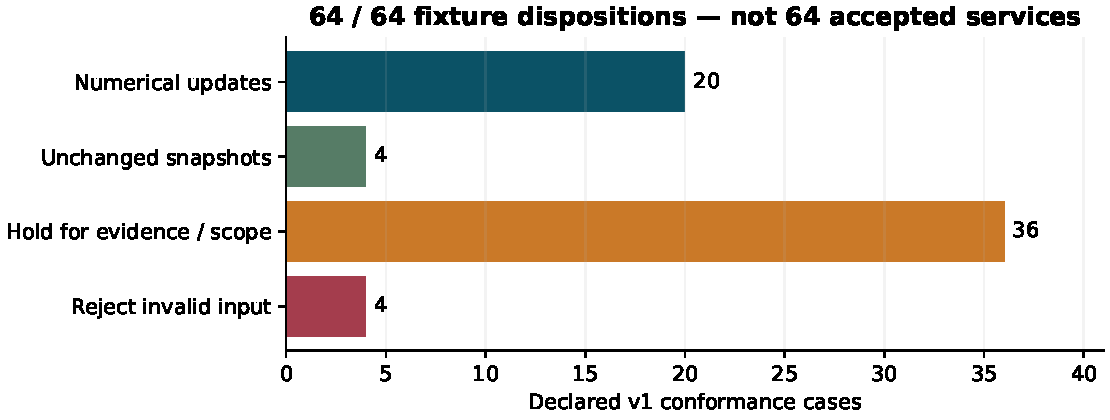
\includegraphics[width=.94\textwidth]{figures/conformance.pdf}
\caption{Preserve the denominator and outcome type. Correct refusal contributes to control conformance but does not manufacture a delivered scientific answer.}
\end{figure}

Thirty repeated timing runs give median conventional full reanalysis of 1.735 ms for writing and 1.574 ms for teacher expectancy. The corresponding unchanged-snapshot paths take 0.261 ms and 0.137 ms. These are local compute timings, excluding reconstruction, source acquisition, agent work, validation and customer effort. They decisively weaken an arithmetic-speed sales story. Any commercial advantage must come from avoided reconstruction, clearer scope, fewer failures or better coordination, all of which need additional measurement.

\subsection{The cheap expertise and transfer assay ties}

\begin{table}[htbp]
\begin{tabularx}{\textwidth}{lrrrrY}
\toprule
Arm & Rubric & Operations & Elapsed(s) & Output(chars) & Execution detail\\
\midrule
U &18/18&6&259.94&$<12000$&Independent Python checks; two failed condensation attempts retained\\
E &18/18&4&281.03&11865&Two numerical formulations; R runtime unavailable\\
E+ &18/18&5&237.27&11754&Verified inherited archive; executed recovered engine and validator\\
\bottomrule
\end{tabularx}
\caption{Observed single sessions. Operation counts normalize the logs: E originally counts four wrappers plus four nested executions as eight calls; these are four execution operations. Elapsed intervals include concurrent host conditions and are not causal latency or cost estimates.}
\end{table}

All three recipients preserve teacher-expectancy meaning, use the supplied effects/variances, flag unresolved dependence and refuse to convert a crop standardized mean difference into kg/ha. Their refusal is an accepted semantic-control answer, not an accepted crop-yield analysis. E+ verifies the frozen archive, executes recovered code on its fresh mapping, and compares the result with an independent analytic score-root calculation. The inherited bytes therefore do useful work; the same observed quality is also achieved by U and E.

The measured rubric differences $E-U$ and $E^+-E$ are both zero. With one small session per arm and no complete cost telemetry, no population effect or cost advantage follows. Nor does this show that expertise is valueless. It shows that this particular cheap checklist and retained artifact did not improve the scored outcomes over competent direct use on these tasks. The workflow is not redefined as Beta after observing the tie. Historical definitions and all effort remain intact.

\subsection{Post-confirmation diagnostics and prospective correction}

A separate reviewer executes nine diagnostic observations and two analytic numerical checks after confirmation. Source/purpose digest drift, missing event kind and malformed authority behave conservatively. Two previously untested conditions expose limits. First, a correction carrying an unrecognized or contradictory \texttt{source\_id}, covariance or dependence field can still recompute because v1 trusts normalized event meaning supplied upstream. Second, a withdrawal followed by another correction is evaluated independently against the original packet: the two outputs have 18 and 19 rows, respectively. The command is an independent snapshot assay, not a chronological ledger.

These are retained adverse findings. The 64-case record is not rewritten to imply those cases were covered. A separate v1.1 candidate tightens the event schema and explicitly rejects sequential mode. Its construction, requirements and generator were frozen at 16:23:08 UTC; new seeded instances were generated at 16:23:13 and executed at 16:23:16. All 46 fresh cases pass. The old 64 cases separately pass regression checks, and 54 preserved file hashes remain unchanged. Its scope remains snapshot revalidation. The correction does not discover external notices, infer dependence, authenticate an issuer or automatically update a historical ledger. Its detailed receipt and new hash are supplied in the evidence companion; the E+ transfer result remains a result for v1, not a retroactive qualification of v1.1.

\subsection{Native controls and comparison boundaries}

The unchanged inherited integration suite passes 29/29 controls. It exercises bytes, cryptography, rights and native accounting under local fixtures. It correctly blocks scientific production admission and prevents unknown actual cost from becoming a profit assertion. The necessary-bound admission diagnostic passes 12 boundary controls, including reachable and impossible cases. The economic ledger's latest 24 controls pass, preserving earlier development corrections.

These counts are different suites, not trials to pool into one headline reliability percentage. Their conjunction makes the research package reviewable. It does not constitute a live protected-network deployment, independent validation of all production behavior or paid-service acceptance. The same-content library control passes 5/5 checks: two separate Python recipients execute the same 32 teacher snapshot cases with identical full outputs. It supplies no graph-specific quality advantage. The isolated recipient processes resolve NumPy 2.3.5, while the original root numerical run used 2.3.2; both use SciPy 1.17.0. This environment difference is recorded rather than described as an exact clean-install reproduction.

\section{The commercial arrangement and its failure conditions}

\subsection{Define the offer before its price}

The proposed initial offer is a bounded reconstruction of one openly accessible quantitative evidence packet. The buyer receives a source/version inventory, effect and variance mapping, executable reproduction, uncertainty and missing-evidence register, and an acceptance record. Editorial decisions, inaccessible primary materials, causality claims and production monitoring are excluded unless separately specified and priced. Automation may do intake, hashing, parsing, calculations, routine verification and packaging. Residual expert work follows actual unresolved obligations; no arbitrary daily review allowance is inserted to predetermine margins.

A comparable human service is the primary commercial reference. This edition obtains no quote. Its explicit planning sensitivity is 4–12 hours at USD 100–200/hour, or USD 400–2400, for the narrow reconstruction/checking scope. These are assumed hours and rates, not market observations or a claim that a complete systematic review costs this amount. A genuinely new continuity contract needs a buyer-value hypothesis, an outside option and actual willingness-to-pay evidence; it cannot borrow a market price merely by naming a new product.

Price is not fixed near token cost. A buyer can accept, decline, defer or use an alternative. The price grid USD 500/800/1200 explores possible quotes, not an optimized price; its demand curve is unknown. A live pricing decision would maximize expected collected contribution subject to participation, acceptance, capacity and cash constraints. Discounts and milestone payments must be justified by changed buyer response, financing or risk, rather than prescribed as 10\% or a fixed reinvestment fraction.

\subsection{Charge each activity once}

\begin{table}[htbp]
\small
\begin{tabularx}{\textwidth}{lYY}
\toprule
Bucket & Included activities & Treatment here\\
\midrule
A: complete delivery & Acquisition, reconstruction, required learning, execution, checks, corrections, failed attempts, agreed support, coordination required by the contract & No actual paid job. Scenario values are assumptions; research labor is not retroactively customer-funded.\\
B: additional retention & Extra assessment, rights review, packaging, admission, transfer, serving overhead and upkeep not already needed for A & Must be deducted once from reusable benefit. No empirical positive monetary admission.\\
C: optional development & Additional Gym practice, R\&D and experiments beyond a promised outcome & This edition's research belongs here in substance; its complete actual monetary cost is unknown.\\
\bottomrule
\end{tabularx}
\caption{Disjoint cost attribution. Unknown actual research cost is not zero. Cash expense and displaced-work opportunity cost are reported separately, not added twice.}
\end{table}

The exact-cent ledger separates capital, deposits, recognized revenue, receivables, collected revenue, refunds, write-offs, costs, supplier payables, reserves and available cash. A later payment of an accrued support cost does not create a second expense. An invoice is not cash. Capital and customer savings are not revenue. A refundable deposit is an obligation until the acceptance condition earns it. An unavailable cost remains unknown; it does not permit a profit claim.

\subsection{Conditional feasibility, not fitted profitability}

Let $n$ be prospective participants, $s$ participation survival, $p$ common technical success probability, $q$ price, $a$ payment probability, $c$ complete per-delivery cost, $G$ coordination cost, and $K$ fixed construction plus additional retention expense. For a simple \emph{no-deposit} threshold model with sunk $K+G$, delivery costs incurred only on technical success and surviving participation, and no residual receipts on payment failure,
\begin{equation}
\mathbb{E}[\Pi]=psn(aq-c)-G-K,\qquad
K_{\max}=psn(aq-c)-G.
\end{equation}
This model makes its simplifying timing/failure structure explicit. It does not describe all contracts. It uses no assumed E+ quality or cost gain, and the unrestricted expert may select the same arrangement. All 135 executed grid values are assumptions propagated exactly: $n\in\{0,1,2,4,6\}$, $q\in\{500,800,1200\}$, $c\in\{100,325,700\}$, $p\in\{1,.9,.7\}$, $s=.9$, $a=.95$, $G=200$.

At $n=4$, $q=800$, $c=325$ and $p=.9$, the fixed-cost ceiling is USD 1,209.40. A strictly smaller $K$ is needed for positive expected contribution; equality merely breaks even. This figure is a decision boundary, not a measured cost, valuation or forecast. At zero participants the ceiling is negative. Raising price raises the ceiling only if participation and collection remain unchanged, an assumption that actual buyers may contradict.

\begin{figure}[htbp]
\centering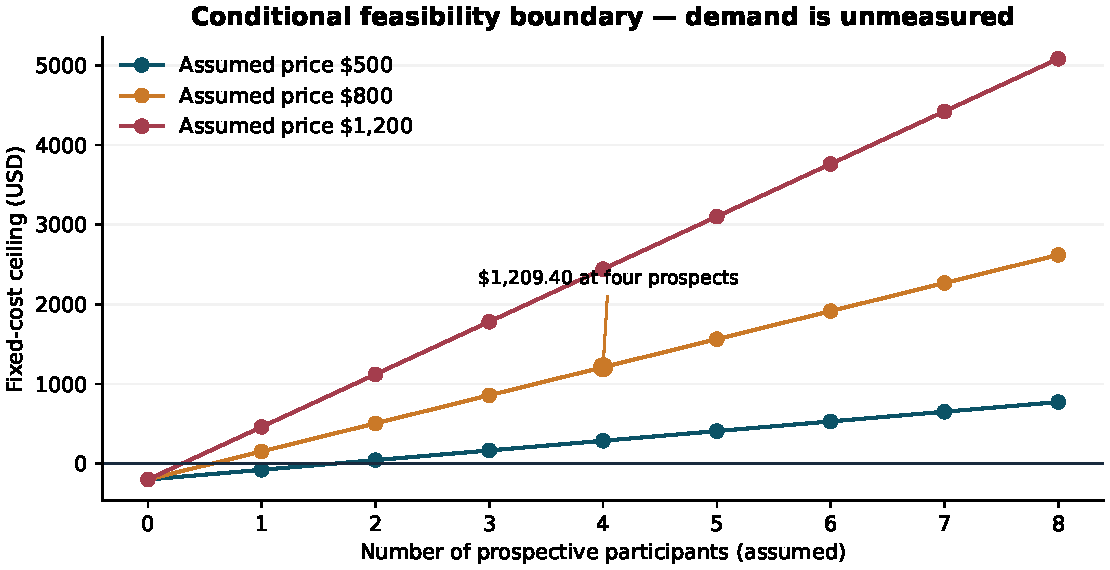
\includegraphics[width=.98\textwidth]{figures/thresholds.pdf}
\caption{Illustrative extension of the exact threshold formula. Every market parameter is assumed: common success 0.9, participation survival 0.9, payment 0.95, complete delivery USD 325 and coordination USD 200. A higher line is not observed demand or an optimized offer.}
\end{figure}

\subsection{Technology and coordination are separate interventions}

The mechanism runner can evaluate no shared capability/no coordination, capability only, coordination only, and both. The study-specific template remains unpriced rather than inserting a guaranteed savings factor. The original supplied Invent-the-Economy example is replayed only as a historical calibration of the ledger: its constructed shared core and buyers are not rediscovered as this opportunity.

For the new opportunity, let $K_0$ and $K_1$ denote fully measured setup costs without and with the retained capability. With $n$ otherwise identical served buyers, coordination costs $G_0,G_1$, and constant delivery terms, the interaction between a shareable setup reduction and pooled demand can have magnitude $(n-1)(K_0-K_1)$ before extra coordination/retention risk. This is algebra conditional on a real shared cost and compatible demand. If $K_0=K_1$, or customer-specific verification dominates, the technical complement disappears. If participants withdraw, a favorable setup amortization can disappear with it.

No value for $K_0-K_1$ is estimated from the millisecond numerical timings or the tied recipient scores. Thus no causal positive technology-by-coordination interaction is claimed here. Giving an expert the same representation, code and contract is required; restricting the expert to one buyer would manufacture the flagship result. The historical restricted 2×2 remains clearly labeled, while an unrestricted expert selects the same feasible package.

\subsection{Cash timing changes the decision}

A separate \emph{deposit-bearing} illustration uses USD 4000 seed capital, a USD 500 protected reserve, four USD 100 refundable deposits, USD 1500 construction, USD 200 coordination, and USD 250 delivery plus USD 75 support per accepted buyer. Each accepted buyer's total price is USD 800. These inputs are hypotheses, not measured human or AI costs. Deposits remain unavailable for construction until earned. All upfront and later costs are charged once to A in this synthetic paid-baseline example; actual research remains C/unknown.

\begin{table}[htbp]
\small
\begin{tabularx}{\textwidth}{Yrrrr}
\toprule
Illustrative path & Final cash & Earned collections & Collected-basis profit & Available funds\\
\midrule
All accepted and paid &4200&3200&200&3700\\
One final-payment default &3500&2500&−500&3000\\
Common technical failure &2300&0&−1700&1800\\
Payment delayed to day 40 &4200&3200&200&3700\\
One withdrawal before delivery &3725&2400&−275&3225\\
Underfunded; only 1000 seed &1400&0&0&500\\
\bottomrule
\end{tabularx}
\caption{US dollars, exact scenario results. The underfunded path stops before construction and still owes 400 in refundable deposits; its cash is not earned surplus. Delay has the same eventual profit but a longer period of unavailable funds. No row is actual revenue.}
\end{table}

\begin{figure}[htbp]
\centering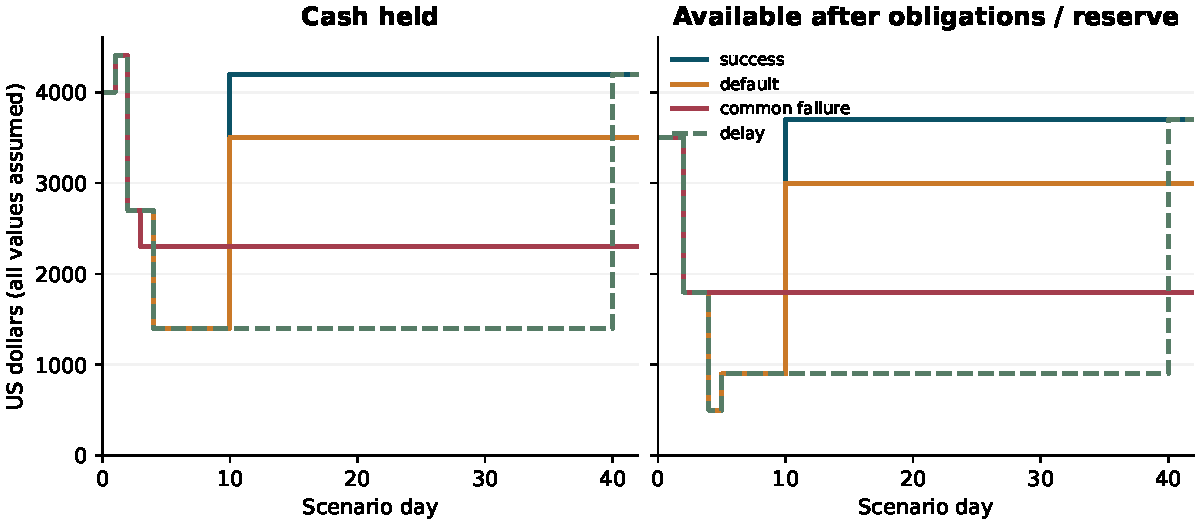
\includegraphics[width=\textwidth]{figures/cash-timing.pdf}
\caption{Cash held differs from cash available after obligations and the protected reserve. The success and delayed-payment paths overlap until the first collection date. The model does not treat receivables as money that can fund new construction.}
\end{figure}

The deposit model's realized paths are not the expectation of the preceding no-deposit formula. Their timing, participation and payment assumptions differ. In particular, the positive USD 200 success contribution does not imply positive expected contribution under technical and payment risk. Neither seed capital nor preserved reserves are counted as earned expansion funds. If a service takes nonrefundable commissioning payments instead, buyer acceptance, rights, delivery obligations and refund law require a separately qualified contract; this study does not assume that change is free.

\section{Selective inheritance, optional practice and authority}

\subsection{Capability lineage}

The lineage has four distinct kinds of contribution. Established statistical methods and source datasets are supplied ingredients. The source-aware adapter and checklist are assistant-constructed generic artifacts. The authenticated capsule and native accounting are inherited repository mechanisms. The recipient constructs its own fresh mapping and checks current semantics. None of these is evidence that the enterprise has learned to invent better.

The v1 correction feedback is recorded as software refinement: original artifact, fixture environment, adverse diagnostic, edit, new version and fresh checks are identifiable. No proprietary weights are modified, no fine-tuning occurs, and no reinforcement-learning score is reported. An optional future Gym campaign could optimize mapping/verification policies across unrelated layouts, incompatible models and source omissions, but only if expected reuse exceeds its cost. Its evaluation must include prompt injection in evidence, false confidence, leakage, negative transfer and obsolete defaults. Correctly declining a campaign can coexist with profitable delivery.

The present candidate may be preserved as research evidence without being admitted as economic Alpha. A useful operational method can later become ordinary Beta as model defaults improve. The baseline and eligible scope must then be updated prospectively; past benefit cannot be counted again under a new name. ``Specialist ASI'' is an ambition, not a description justified by this small pilot.

\subsection{Admission must be possible, then earned}

An unchanged admission policy requires 6–24 paired independent mission clusters, a positive one-sided 95\% lower bound, and positive lower-bound lifetime net benefit after assessment and lifecycle costs. Candidate identity, comparator, policy, scope, environment, times and prerequisites must match. This edition supplies no such empirical monetary evidence, so no positive admission follows from control conformance.

A necessary prescreen can avoid structurally impossible assessments. If the maximum benefit per eligible reuse is $M$, risk reserve per use is $S$, eligible reuse forecast is $R$, assessment expense is $A$ and additional lifecycle expense is $L$, then an upper bound on admissible lifetime value is
\begin{equation}
U=(M-S)R-A-L.
\end{equation}
If even $U$ cannot clear the policy hurdle, no favorable sample can do so under those bounds. Passing this prescreen merely means assessment could be informative. It is not evidence of realized benefit, valid reuse forecasts, correctness or permission. Twelve local boundary controls validate the necessary-bound computation. Nine additional economic cases explore reachable and impossible assumptions without assigning a positive measured lower bound.

The earlier corrected-study notice reports 568 assessment states whose capped benefits cannot reach their final hurdles, with maximum ratios 73.016\% in the reference profile and 78.971\% in a favorable profile. Its assessment expenses remain USD 261.56 and USD 1335.94 per network world. Those are preserved post-confirmation diagnostics from the notice, not rerun measurements or recovered profit. The complete private paper and ledgers were not retrieved.\citep{advantage} Any changed prescreen must be frozen and tested prospectively; different timing can change later cash, workload and opportunities.

\subsection{Protected sharing without inherited permission}

The intended network makes admitted, rights-cleared generic capabilities available to currently authorized \texttt{*.agent.agi.eth} members through existing protected interfaces. Current membership, revocation, Jobs validator roles, execution authority and settlement remain separate checks. Wildcard naming is not proof of identity. A prior success, graph node or surviving local copy cannot revive expired permission.

Source secrets, restricted IP and protected evaluation answers must remain outside shared capsules. Here original sources stay under their own licenses and the generic archive excludes them. Revocation can stop later mediated retrieval; it cannot erase an already delivered copy. Requalification follows changes in the model, source, purpose, schema, rights or relevant economic baseline. The present fixture proves neither live ENS authentication nor admission into a production scientific service.

\section{What the successor can do next}

\subsection{A productive frontier with an explicit null result}

Define a feasible offering before comparing configurations: the original useful output is accepted, complete expected contribution is positive, obligations and reserves are fundable at every payment date, serving capacity is sufficient, rights and authority are current, and agreed turnaround/customer-effort limits are met. If both configurations satisfy this envelope, a difference is better economics or reliability, not newly feasible work.

The present evidence establishes no offering that passes this envelope only under E+. Conditional numerical reproduction and semantic diagnosis are available to U, E and E+. A complete crop-yield answer passes for none. Live cumulative monitoring, validated editorial decisions and positive commercial continuity contracts remain unqualified. No measured customer set expands and cumulative incremental commercial net value remains unknown; observed customer revenue is zero.

What the successor does inherit is concrete: executable generic calculations, a small operation checklist, provenance and rights boundaries, transferable bytes, the fresh teacher mapping, adverse cases, a stricter snapshot candidate, exact cash accounting and a necessary admission-feasibility test. Those assets make additional questions executable. Their preservation is justified as research provenance in this edition, not by an invented positive return on future reuse.

\begin{table}[htbp]
\small
\begin{tabularx}{\textwidth}{YYY}
\toprule
Next question & Current asset & Evidence still required\\
\midrule
Can a legacy conclusion be reconstructed cheaply? & Source contract, validator and conventional engine & Unfamiliar messy packets without supplied extraction; metered full cost versus H and E\\
Can continuity survive real changes? & Frozen snapshots and prospective strict schema & Independent notice coverage, chronological/idempotent ledger, real amendments and controlled omission tests\\
Can shared construction finance delivery? & Exact ledger, participation and threshold model & Binding buyer choices, actual shared work, complete costs, refund/default/support terms and funding\\
Does inheritance broaden the mission? & Teacher transfer and incompatible-crop refusal & New compatible missions with preserved purpose and quantified adaptation; neither cherry-picked demand nor hidden answers\\
Should the enterprise build another instrument? & Reachability bound, cost buckets and stop rules & Positive incremental expected value after all R\&D, retention and opportunity costs; current cash available\\
\bottomrule
\end{tabularx}
\caption{The next frontier is a sequence of testable decisions, not a larger hypothetical market inferred from graph growth.}
\end{table}

\subsection{Operating blueprint}

\textbf{Offer.} Begin with the narrow source-qualified reconstruction or a clearly priced missing-evidence assessment. Identify a specific synthesis owner and its outside option. Obtain an equivalent human quote or a defensible activity estimate for the same scope. A diagnostic refusal must have been valuable under the original contract; it is not relabeled as success afterward.

\textbf{Deliver expertly.} Freeze the question, units, study identity, admissibility policy, uncertainty model, evidence access and acceptance. Automate inventory and reproducible calculations. Use current suitable frontier models to inspect and reconcile meaning, execute conventional tools, challenge the mapping and correct failures. Record retries, model/tool usage, operator and customer effort, source delay and actual support. Independent checks must not reuse the same mistaken assumption as the producer.

\textbf{Construct.} Build only the generic structure needed to serve a real task family: extraction adapters where rights allow, source/effect/model contracts, missing-information requests and executable checks. A live continuity extension must bind ordered events to updated packet hashes, handle idempotency and reinstatement, verify source coverage, and refuse incompatible changes. These are engineering requirements, not already executed production features.

\textbf{Retain.} Separate paid-delivery work from extra qualification/generalization. Apply the necessary feasibility bound before expensive assessment. Preserve rejected candidates and their expense. Admit only after fresh semantic, rights, authority and incremental-value evidence; otherwise retain research receipts without broadcasting a qualified specialist. Use an ordinary library as the same-content counterfactual.

\textbf{Coordinate and finance.} Seek co-commissioning only where customers actually share cleared work. Make the funding threshold, milestones, ownership/licenses, responsibilities, withdrawal consequences, refunds and common-failure response explicit. Do not spend refundable funds or invoices. Model collection timing and capacity during correlated correction bursts. Compare production, exploration, assessment, optional practice, specialist invocation, sharing, preserving cash and stopping without requiring a fixed number of investments.

\textbf{Expand or stop.} Expansion requires earned surplus after liabilities/reserves, accepted quality on unfamiliar work and positive complete incremental value. Stop when participation is too small, adaptation destroys the setup saving, the human/expert alternative already fits the envelope, source rights or evidence are unavailable, defaults exhaust liquidity, or improved model defaults erase the operational advantage. More agents or jobs at larger budgets would not establish compounding.

\section{Current frontier models and actual execution provenance}

Official documentation checked on 27 October 2026 identifies \texttt{gpt-6-astra} for demanding reasoning/research/code work and \texttt{gpt-6.1-terra} for efficient visual reasoning and precise computer use. Both list a 1,050,000-token context and 128,000 maximum output. Astra lists low through max reasoning effort; Terra also lists none and requires the Responses API for tool calling. These are suitable role candidates, not fixed restrictions on future successors.\citep{astra,terra}

Standard listed text-token prices are USD 10/50 per million input/output for Astra and USD 1/5 for Terra. With assumed 60000 input and 10000 output tokens, token charges alone would be USD 1.10 and USD 0.11. These are sensitivity calculations, not this study's invoices. Tools, cache behavior, retries, reasoning/output usage, verification, orchestration, customer effort and support still matter. Long-context and service-tier adjustments apply; account-specific access/rate limits were not verified. ChatGPT Pro is a plan, not an API model identifier or an automatic entitlement.\citep{astra,terra,pricing}

The actual research uses available assistant reasoning, delegation, browsing, code execution and local validation. It does not substitute deterministic logic for a frontier-model efficacy trial: deterministic conformance is reported as such, while the three assistant sessions are actual but small and unmetered. There are no paid API calls claimed, human trials, sales or live production identity actions. Neither official model name establishes the exact billing configuration of the internal sessions.

\section{Limitations, publication and conclusion}

The most important limitation is the distance between a source-qualified snapshot calculation and an economically viable continuity service. Supplied secondary data simplify reconstruction. Both numerical datasets were known to the constructor. Explicit event kinds simplify interpretation. Public-source ambiguities remain unresolved. Reviewer and recipients are AI agents with procedural separation. The sample cannot estimate representative user behavior, rare semantic failure or service reliability. No customer effort, full research cost, human equivalent quote or willingness to pay is observed. Conditional cash scenarios and any future simulation intervals cannot validate those assumptions.

The study nevertheless contributes an inspectable experiment and a disciplined rejection of stronger claims. Source meanings survive one actual recipient transfer; incompatible reuse is refused; conventional experts remain strong; a failed diagnostic remains visible; monetary unknowns do not become profit; production authority does not follow from an artifact. These outcomes improve the enterprise's evidence and test apparatus without proving learning-to-invent or a commercial flywheel.

Publication remains additive. Immutable source versions, all failed/adverse observations, original v1 bytes, prospective corrections, raw result files and licensed source notices are delivered with the LaTeX/PDF, evidence companion, executive brief and English/French browser demonstration. The existing repository paper process and issue 4850 owners govern public deployment. New executable HTML requires full source qualification; a draft source handoff or asset hash is not a verified live paper-reader release. No alternate hosting path, production scope or reserved software version is appropriated.\citep{paperpolicy}

The practical next step is small: one unfamiliar, rights-cleared legacy packet whose owner values a defined outcome, a fair human/expert alternative, complete activity metering and fresh acceptance. If that test fails, stop or change the opportunity. If it succeeds, evaluate compatible recurrence and financing before sharing or expanding. The successor should inherit useful structure and the reasons it can fail, while earning each new acceptance and authority.

\appendix
\section{Preserved historical quantities and corrections}

The original Invent-the-Economy example has four synthetic buyers paying USD 300000 on success, each valuing the outcome at USD 360000, delivery cost USD 75000 each, common construction USD 600000 and technical success probability 0.8. Successful contribution is USD 300000. Common failure loses USD 600000. Expected contribution is USD 120000. Required opening cash is USD 900000 because construction and delivery precede payment. These quantities are different. A USD 40000 route cost per delivered buyer makes expected contribution negative USD 8000.\citep{economy}

The example's first success leaves USD 300000 earned surplus above the protected seed reserve. A subsequent two-buyer setup costing USD 300000 has positive expected contribution USD 60000 but requires USD 450000 prefunding, so cannot be funded from that surplus. A supplied USD 150000 setup needs USD 300000 opening cash and has expected contribution USD 210000. These are alternate assumed learning conditions, not observed costs or autonomous market creation.

The Harness's conventional sweep/prefix example reports producer counts 67512 versus 3977, while checker counts change 12076 to 28612. The operation models are distinct and cannot be added as dollars. Its polynomial task is multiplication/coefficient convolution, not substitution; learned continuation takes 207 checks versus expert 183 and 297 after 90 additional qualification checks. Historical thermal results retain their failed acceptance and stronger baseline corrections. These are source-audited history, not silently superseded by this edition's experiment.\citep{harness,repository}

\section{Evidence classes and reproducibility map}

\begin{longtable}{>{\raggedright\arraybackslash}p{.18\textwidth}p{.75\textwidth}}
\toprule
Class & Meaning in this edition\\
\midrule\endhead
Observed & Executed local code/bytes, numerical outputs, elapsed logs, saved answers, conformance and adverse diagnostic results. Observation of a simulated fixture does not turn its premises into real identities or demand.\\
Sourced & Public documents, source code, secondary data, official model specifications and historical correction notices. Commit and content receipts identify immutable sources where available. Mutable web pages are dated retrievals, not guaranteed future versions.\\
Calibrated & No market or model-performance parameter is fitted to observations. The historical synthetic mechanism is a reference replay, not empirical calibration.\\
Assumed & Price, demand, human hours/rates, common success, participation, payment, delivery cost, support and reserves in economic examples.\\
Simulated & Counterparties, ENS principals, access evidence used to reach test branches, injected events and conditional commercial paths.\\
Unmeasured & Actual complete cost/profit, representative quality differences, genuine buyer acceptance, customer effort, live authentication, newly feasible commercial work and cumulative net commercial value.\\
\bottomrule
\end{longtable}

The reproduction entrypoint is the study README. \texttt{run\_study.py} reproduces the numeric suite to a new output directory. \texttt{integration/run\_controls.py} invokes the unchanged predecessor closure; \texttt{integration/library\_equality.py} compares identical content. \texttt{economics/check\_invariants.py} and \texttt{economics/thresholds.py} reproduce accounting and conditional boundaries. Protocol freezes precede their relevant executions. Recipient answers, source coordinates, timestamps, retries and review receipts remain separate. The prospective correction has its own runner and freeze. Full repository CI/hosted qualification is not replaced by these scoped checks.

New generic code is Apache-2.0. Source files retain their GPL/AGPL and other original notices; no single-license claim is made for the bundle. The artifact archive deliberately excludes those datasets. AI systems assisted research, analysis, implementation, review, translation and drafting. The specified author attribution does not assert that the named author independently executed or personally reviewed every check. Final scholarly/editorial approval remains with the author and repository owners.

\clearpage
\bibliographystyle{unsrtnat}
\bibliography{references}
\end{document}
